
% ------------------------------------------------------------
% ------------------------------------------------------------

\section[Summary Plots]{Summary Plots}

%%%%%%%%%%%%%%%%%%%%%%%%%%%%%%%%%%%%%
\subsection{Basic Plots}
%%%%%%%%%%%%%%%%%%%%%%%%%%%%%%%%%%%%%
\begin{frame}[fragile, allowframebreaks]
  \frametitle{Basic Plot}
      
      		\begin{lstlisting}
			# Step 1: Load the Data
			library(alr3)
			data(UN2)
			attach(UN2)
			# Step 2: Subset appropriately
			ind<-which(Purban>50)
			# Step 3: Plot		
			plot(logFertility~logPPgdp, xlab="logPPgdp", ylab="logFertility", main="logGDP vs logFertility Plot")
			points(logFertility[ind]~logPPgdp[ind], col="red", pch=19)
			legend("topright", pch=c(1,19), col=1:2, c("Purban<50", "Purban>=50"))
		\end{lstlisting}
%
\newpage
       \begin{center}
         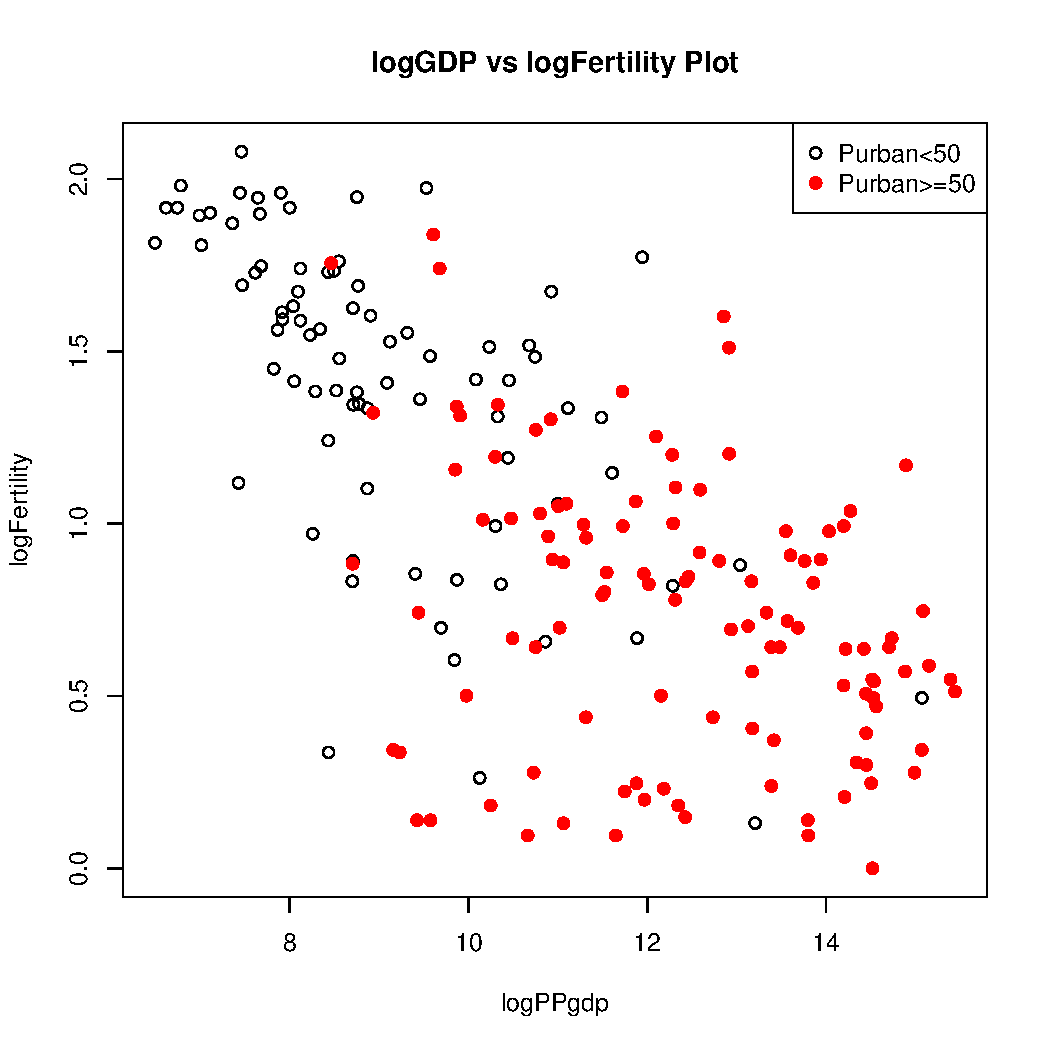
\includegraphics[width=0.65\textwidth]{images/Unplot3.pdf}
        \end{center}


\end{frame}

%____________
\begin{frame}[fragile, allowframebreaks]
  \frametitle{Segmented bar charts}

Displays two categorical variables at a time: \footnote{These two slides are modified from the SCC Mini-Course "Introductory Statistics with R" by Mine \c{C}etinkaya}

\tiny
\begin{lstlisting}
survey = read.table("http://www.stat.ucla.edu/~mine/students_survey_2008.txt", header = TRUE, sep = "\t")
attach(survey)
barplot(table(gender, hand), col = c("skyblue", "blue"), main = "Segmented Bar Plot \n of Gender")
legend("topleft", c("females","males"), col = c("skyblue", "blue"), pch = 16, inset = 0.05)
\end{lstlisting}

\newpage
    \begin{columns}
      \column{0.50\textwidth}
      
       \begin{center}
\includegraphics[width = 53mm]{images/segbarplot.pdf}
\end{center}

     \column{0.50\textwidth}
\begin{center}
\scalebox{1.2}{%
\begin{tabular}{|r|r|r|r|}
  \hline
 & ambidextrous & left & right \\ \hline
  \hline
female &   9 &  67 & 806 \\ 
  male &  11 &  45 & 387 \\ 
   \hline
\end{tabular}}
\end{center}
\normalsize
\end{columns}

\end{frame}

%_______________________
\begin{frame}[fragile, allowframebreaks]
  \frametitle{Dot charts}

To compare values for variables in each category:

\begin{lstlisting}
# Step 1: Load the data
data(iris)
attach(iris)
# Step 2: Calculate means for each species:
aggregate(iris[, -5], list(Species = Species), mean)->a
# Step 3: Assign row names
row.names(a)<-a[, 1]
# Step 4: Plot
dotchart(t(a[, -1]), xlim = c(0,10), main="Plots of Means for Iris Data Set", xlab="Mean Value")
\end{lstlisting}

\newpage
       \begin{center}
		\includegraphics[width = 70mm]{images/dotPlot.pdf}
	\end{center}

\end{frame}

%%%%%%%%%%%%%%%%%%%%%%%%%%%%%%%%%%%%%
\subsection{Looking at Distributions}
%%%%%%%%%%%%%%%%%%%%%%%%%%%%%%%%%%%%%

\begin{frame}[fragile]
\frametitle{Histograms}
  \framesubtitle{Adding Summary Statistics to Plots}
Add the mean and median to a histogram:
    \begin{columns}
      \column{0.61\textwidth}

\begin{lstlisting}
hist(ageinmonths, main="Histogram of Age (Mo)")
abline(v=mean(ageinmonths), col = "blue", lwd=3)
abline(v=median(ageinmonths), col = "red", lwd=3)
legend("topright", c("Mean", "Median"), pch = 16, col = c("blue", "red"))
\end{lstlisting}

     \column{0.39\textwidth}
\begin{center}
\includegraphics[width = 45mm]{images/hist_meanmed.pdf}
\end{center}

\end{columns}
\end{frame}

%%%%% New frame
\begin{frame}[allowframebreaks, fragile]
\frametitle{Histograms}
\framesubtitle{Checking Normality}

One of the methods to test for normality of a variable is to look at the histogram (the sample density is in red, the theoretical normal density in blue):
  		\begin{lstlisting}
data(presidents)		
hist(presidents, prob=TRUE, ylim=c(0, 0.04), breaks=20)
lines(density(presidents, na.rm=TRUE), col="red")
mu<-mean(presidents, na.rm=TRUE) 
sigma<-sd(presidents, na.rm=TRUE)
x<-seq(10,100,length=100) 
y<-dnorm(x,mu,sigma) 
lines(x,y,lwd=2,col="blue") 
		\end{lstlisting}

        \begin{center}
         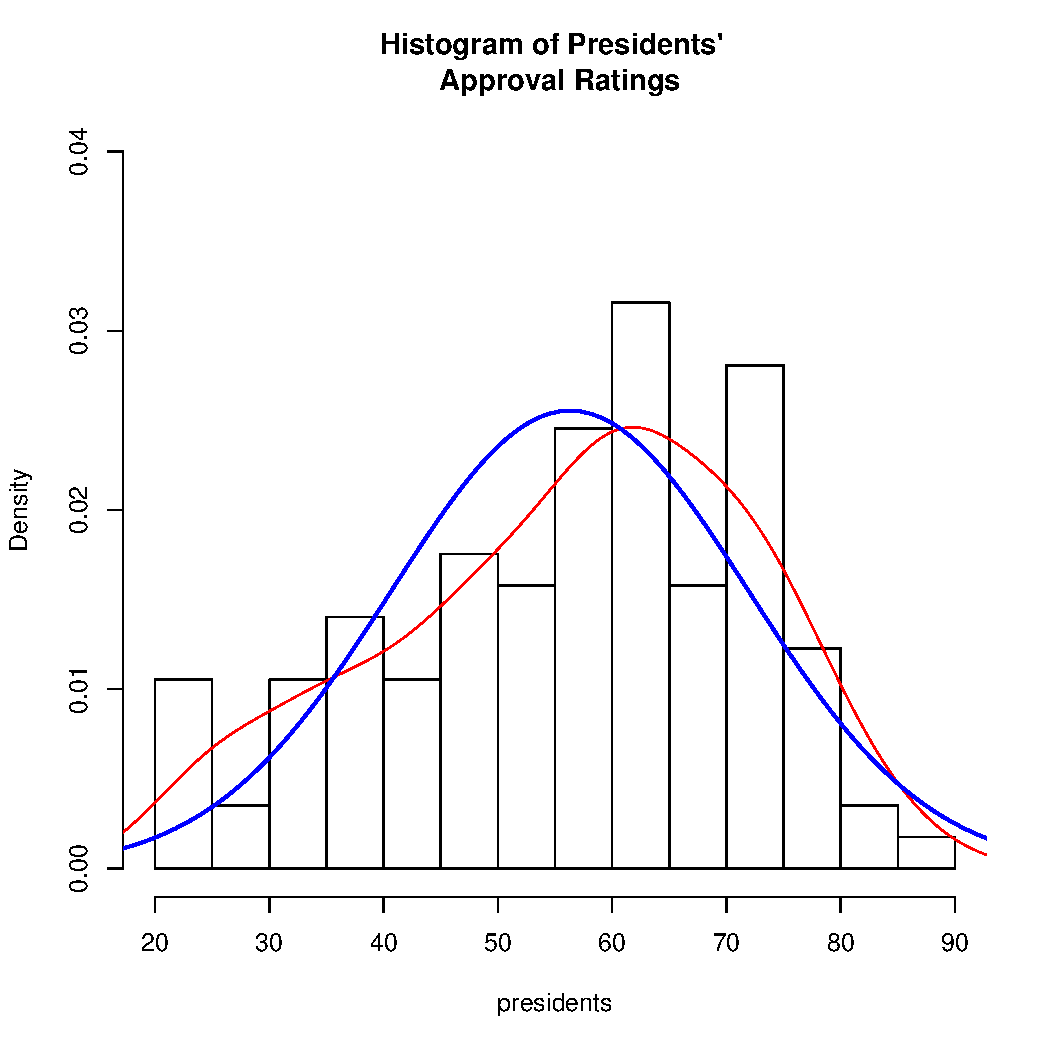
\includegraphics[width=0.6\textwidth]{images/presHist.pdf}
        \end{center}
\end{frame}


%%%%% New frame
\begin{frame}[allowframebreaks, fragile]
\frametitle{Box and Whisker Plot}

Another method of looking at the distribution of the data is via boxplot:
  		\begin{lstlisting}
data(quakes)		
# Subset the magnitude:
ind<-ifelse(quakes$mag<4.5, 0, 1)
ind<-as.factor(ind)
library(lattice)
bwplot(quakes$mag~ind, xlab=c("Mag<4.5", "Mag>=4.5"), ylab="Magnitude")
		\end{lstlisting}
%boxplot(quakes[, 4]~ind)
%# Alternatively:

        \begin{center}
         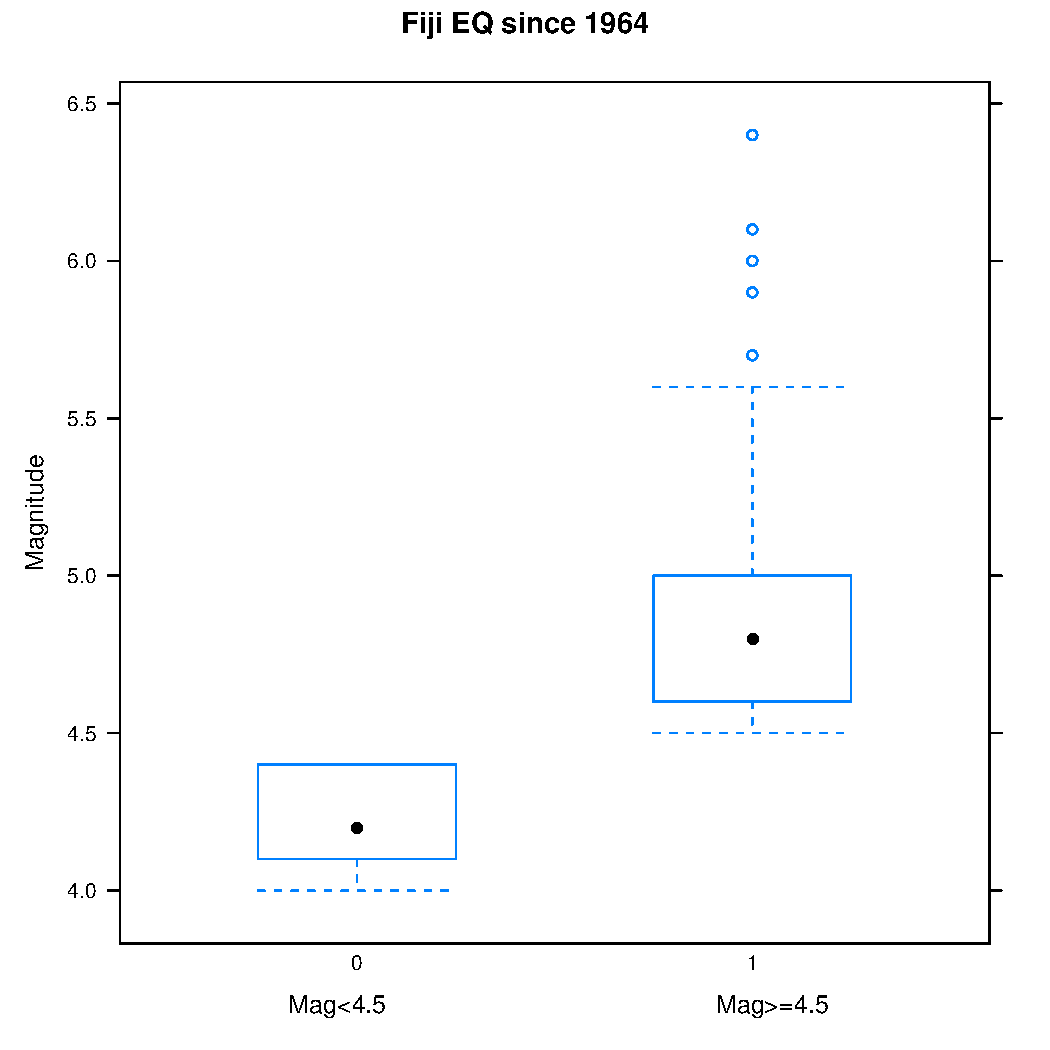
\includegraphics[width=0.6\textwidth]{images/bwplot.pdf}
        \end{center}
\end{frame}

%%%%%% Alternatively:
\begin{frame}[allowframebreaks, fragile]
\frametitle{Beanplot}

An alternative to the boxplot is the  \ttfamily beanplot(): \normalfont
  		\begin{lstlisting}
library(beanplot)		
par(mfrow=c(1,2))
data(airquality)
boxplot(airquality[, 2], main="Boxplot", xlab="Solar")
beanplot(airquality[, 2], main="Beanplot", xlab="Solar")
		\end{lstlisting}
%For documentation of the package, please see: \itshape{\urlwofont{http://www.jstatsoft.org/v28/c01/}}.
        \begin{center}
         \includegraphics[width=0.7\textwidth]{images/beanPlot.pdf}
        \end{center}
\end{frame}
% left-skew: mean to the left of median

%%%%% New frame
\begin{frame}[allowframebreaks, fragile]
\frametitle{Scatterplots}

A method of looking at the distribution and correlation of the data is via \ttfamily scatterplot.matrix(): \normalfont
  		\begin{lstlisting}
data(quakes)
library(car)		
scatterplot.matrix(quakes[, 1:4])
		\end{lstlisting}

        \begin{center}
         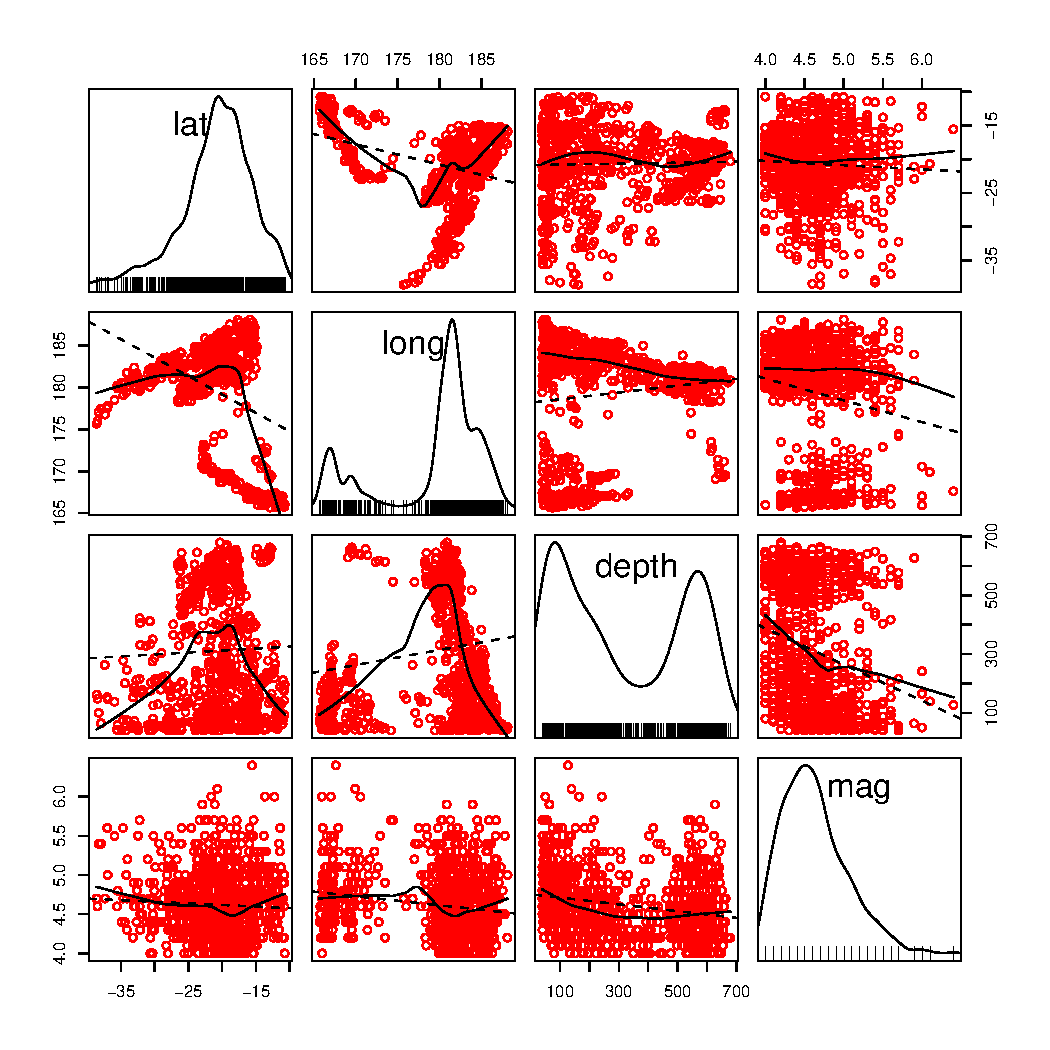
\includegraphics[width=0.63\textwidth]{images/scatterPlot.pdf}
        \end{center}
\end{frame}

%%%% Check equality of distributions:
\begin{frame}[allowframebreaks, fragile]
\frametitle{Checking Equality of Distributions}
\framesubtitle{Approach 1}

A method of checking equality of distributions is via \ttfamily qq(): \normalfont
  		\begin{lstlisting}
library(lattice)
survey = read.table("http://www.stat.ucla.edu/~mine/students_survey_2008.txt", header = TRUE, sep = "\t")
attach(survey) 
qq(gender~ageinmonths)
		\end{lstlisting}

        \begin{center}
         
\includegraphics[width=0.6\textwidth]{images/qq.png}
        \end{center}
\end{frame}

%%%%% New frame
\begin{frame}[allowframebreaks, fragile]
\frametitle{Checking Equality of Distributions}
\framesubtitle{Approach 2}

Another method for checking equality of distributions is via \ttfamily beanplot(): \normalfont

	\begin{lstlisting}
		survey = read.table("http://www.stat.ucla.edu/~mine/students_survey_2008.txt", header = TRUE, sep = "\t")
		attach(survey)
		beanplot(ageinmonths ~ gender, data=survey, col=list(grey(0.5),c(grey(0.8),"white")), border = NA, overallline = "median", ll=0.01, side="both")
		legend("bottomleft",fill=c(grey(0.5),grey(0.8)), legend=c("Female","Male"))
	\end{lstlisting}
	
        \begin{center}
	         \includegraphics[width=0.65\textwidth]{images/beanplotSurvey.png}
        \end{center}
\end{frame}

%split.screen(c(1,2))        # split display into two screens
%split.screen(c(2,1),2)      # split bottom half in two
%screen(1)                   # prepare screen 1 for output
%qq(gender~ageinmonths)
%screen(4)                   # prepare screen 4 for output
% # boxplot(ageinmonths~gender)
% beanplot(ageinmonths~gender, ll=0.04, log="", col="black")
%screen(1, FALSE)            # return to screen 1, but do not clear
%close.screen(all = TRUE)    # exit split-screen mode

%_______________________
\subsection{\ttfamily Identify\normalfont-ing Observations}
%%%%%%% New frame
\begin{frame}[fragile, allowframebreaks]
\frametitle{\ttfamily Identify\normalfont-ing Observations}
\framesubtitle{Preliminaries}
	\begin{lstlisting}
		# Generate data and fit a regression curve:
		set.seed(3012008)
		x=rnorm(100); y=-x+I(x^2) +rnorm(100)
		fit<-lm(y~x+I(x^2)); fit
	\end{lstlisting}

\begin{center}
\scalebox{1}{%
\begin{tabular}{|r|r|r|}
  \hline
 Intercept & x & $x^2$ \\
  \hline
0.1307 & -0.9701 & 0.9549  \\ 
   \hline
\end{tabular}}
\end{center}
\normalsize

	\begin{lstlisting}
		# Plot the resulting regression curve:
		plot(y~x, pch=19)
		curve(expr=fit[[1]][1]+fit[[1]][2]*x+fit[[1]][3]*I(x^2), from=range(x)[1], to=range(x)[2], add=TRUE, col="blue", lwd=2)
	\end{lstlisting}

\newpage
\begin{center}
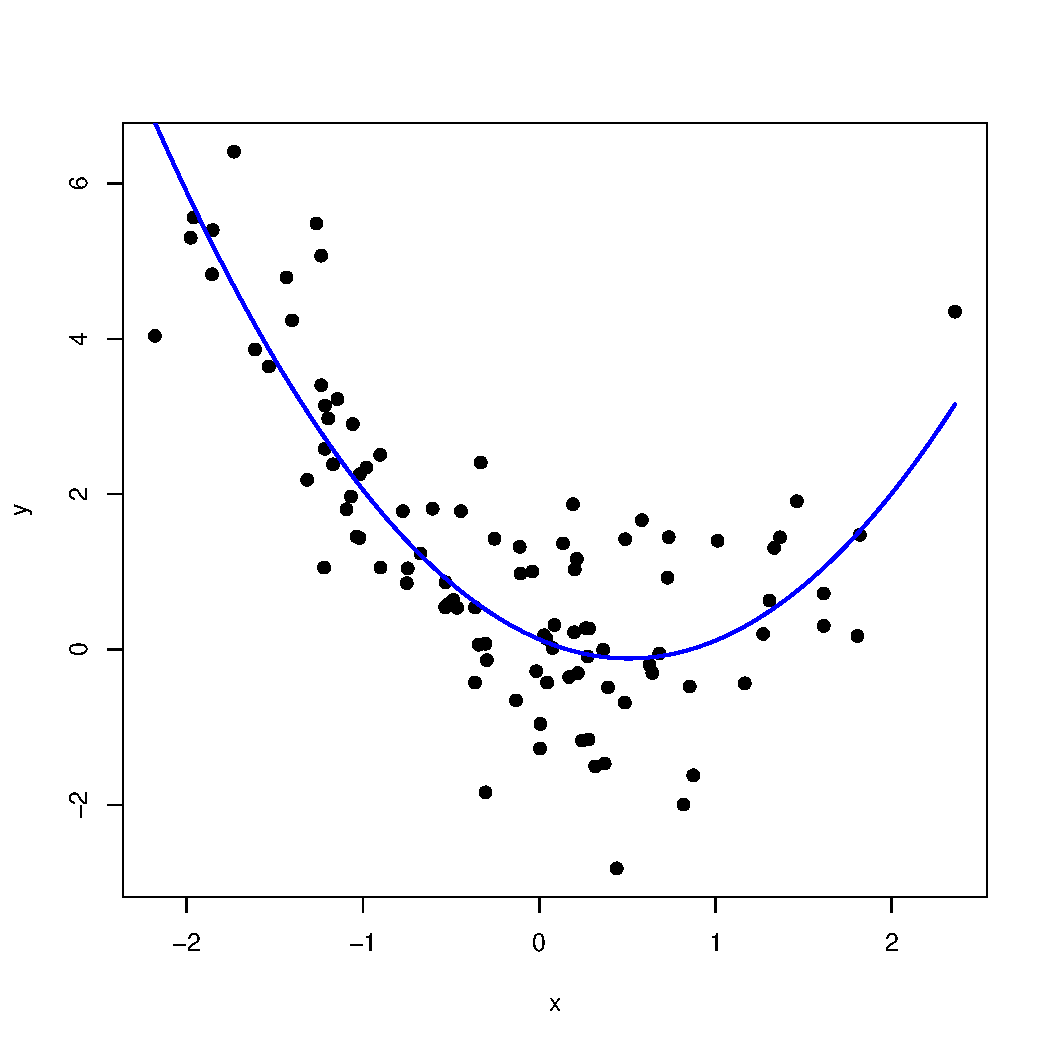
\includegraphics[scale=0.35]{images/xyPlot.pdf}
\end{center}

\end{frame}

%%%
\begin{frame}[fragile, allowframebreaks]
\frametitle{\ttfamily Identify\normalfont-ing Observations}
\textbf{Left-click} \normalfont on the observations in the graphics window to see the row number. \\
\noindent \textbf{Right-click} \normalfont on the observation to exit the function.
	\begin{lstlisting}
		# Plot the data and fit the regression curve:
		plot(y~x, pch=19)
		curve(expr=fit[[1]][1]+fit[[1]][2]*x+fit[[1]][3]*I(x^2), from=range(x)[1], to=range(x)[2], add=TRUE, col="blue", lwd=2)
		# Identify the "outlying" observations:
		index<-identify(y~x); index		
	\end{lstlisting}

\newpage
\begin{center}
\includegraphics[scale=0.27]{images/xyPlotInd.png}
\end{center}

\end{frame}



%%%%%%%%%%%%%%%%%%%%%%%%%%%%%%%%%%%%%

% ------------------------------------------------------------
% ------------------------------------------------------------

% Exercise: compare distributions of Iris data
% ID outlier in dataset

\subsection{Exercise I}
\begin{frame}
	\frametitle{Exercise I}
	Compare the distributions of the sepal widths for the three species of irises (using the \ttfamily iris \normalfont data set).
\end{frame}